% verso e anverso:
% \documentclass[12pt,openright,twoside,a4paper,english]{abntex2}
% apenas verso: 
\documentclass[12pt,oneside,a4paper,english]{abntex2}


\usepackage{cmap}				% Mapear caracteres especiais no PDF
\usepackage{lmodern}			% Usa a fonte Latin Modern			
\usepackage[T1]{fontenc}		% Selecao de codigos de fonte.
\usepackage[utf8]{inputenc}		% Codificacao do documento (conversão automática dos acentos)
\usepackage{lastpage}			% Usado pela Ficha catalográfica
\usepackage{indentfirst}		% Indenta o primeiro parágrafo de cada seção.
\usepackage{color}				% Controle das cores
\usepackage{graphicx}			% Inclusão de gráficos
\usepackage{pdfpages}
\usepackage[brazilian,hyperpageref]{backref}	 % Paginas com as citações na bibl
\usepackage[alf]{abntex2cite}	% Citações padrão ABNT

\usepackage{listings}
\usepackage{color}
\usepackage{float}

\definecolor{mygreen}{rgb}{0,0.6,0}
\definecolor{mygray}{rgb}{0.5,0.5,0.5}
\definecolor{mymauve}{rgb}{0.58,0,0.82}

\lstdefinelanguage{rock}
{
  morekeywords ={const, typedef, tipo, struct, begin, end, inteiro, function, program, if, then, else, while, do, scan, print, int, float, void, char, bool},
  sensitive = true,
  morecomment = [s]{\%}{\%},
  morestring = [b]",
}

\lstset{ %
  backgroundcolor=\color{white},   % choose the background color; you must add \usepackage{color} or \usepackage{xcolor}
  basicstyle=\footnotesize,        % the size of the fonts that are used for the code
  breakatwhitespace=false,         % sets if automatic breaks should only happen at whitespace
  breaklines=true,                 % sets automatic line breaking
  captionpos=b,                    % sets the caption-position to bottom
  commentstyle=\color{mygreen},    % comment style
  deletekeywords={...},            % if you want to delete keywords from the given language
  escapeinside={\%*}{*)},          % if you want to add LaTeX within your code
  extendedchars=true,              % lets you use non-ASCII characters; for 8-bits encodings only, does not work with UTF-8
  frame=single,                    % adds a frame around the code
  keepspaces=true,                 % keeps spaces in text, useful for keeping indentation of code (possibly needs columns=flexible)
  keywordstyle=\color{blue},       % keyword style
  language=rock,
  numbers=left,                    % where to put the line-numbers; possible values are (none, left, right)
  numbersep=5pt,                   % how far the line-numbers are from the code
  numberstyle=\tiny\color{mygray}, % the style that is used for the line-numbers
  rulecolor=\color{black},         % if not set, the frame-color may be changed on line-breaks within not-black text (e.g. comments (green here))
  showspaces=false,                % show spaces everywhere adding particular underscores; it overrides 'showstringspaces'
  showstringspaces=false,          % underline spaces within strings only
  showtabs=false,                  % show tabs within strings adding particular underscores
  stepnumber=1,                    % the step between two line-numbers. If it's 1, each line will be numbered
  stringstyle=\color{mymauve},     % string literal style
  tabsize=2,                       % sets default tabsize to 2 spaces
  title=\lstname                   % show the filename of files included with \lstinputlisting; also try caption instead of title
}

% Configurações do pacote backref
% Usado sem a opção hyperpageref de backref
\renewcommand{\backrefpagesname}{Citado na(s) página(s):~}
% Texto padrão antes do número das páginas
\renewcommand{\backref}{}
% Define os textos da citação
\renewcommand*{\backrefalt}[4]{
	\ifcase #1 %
		Nenhuma citação no texto.%
	\or
		Citado na página #2.%
	\else
		Citado #1 vezes nas páginas #2.%
	\fi}%

\definecolor{blue}{RGB}{41,5,195} % alterando o aspecto da cor azul

\makeatletter
\hypersetup{
     	%pagebackref=true,
		pdftitle={\@title}, 
		pdfauthor={\@author},
    	pdfsubject={\@title},
		pdfkeywords={Compiladores}, 
		colorlinks=true,       		% false: boxed links; true: colored links
    	linkcolor=blue,          	% color of internal links
    	citecolor=blue,        		% color of links to bibliography
    	filecolor=magenta,      		% color of file links
		urlcolor=blue,
		bookmarksdepth=4
}
\makeatother

\autor{Alan D. Barroso, Kenji Sakata Jr}
\title{Anlisador Sintático}
\orientador[]{Linguagens e Compiladores \\ PCS2056}
\instituicao{%
	Universidade de São Paulo
	\par
	Escola Politécnica}
\local{São Paulo}
\data{2013}

\setlrmarginsandblock{4cm}{4cm}{*}
\setulmarginsandblock{4cm}{4cm}{*}
\checkandfixthelayout

\setlength{\parindent}{1.3cm} % O tamanho do parágrafo
\setlength{\parskip}{0.2cm}  % Controle do espaçamento entre um parágrafo e outro

\SingleSpacing

\makeindex

\begin{document}

\frenchspacing % Retira espaço extra obsoleto entre as frases.

\imprimirfolhaderosto

\clearpage

\textual

\chapter{Introdução}

  O analisador sintático é o responsável por reconhecer a estrutura da linguagem, formada a partir da gramática. Sua ação começa uma vez que o módulo léxico já reconheceu todas as partículas átomicas que compõem o código-fonte.


  Na realidade, é o analisador sintático quem invoca a ação do módulo léxico em um primeiro momento a fim de identificar as partículas do texto. Em seguida, ele, o analisador sintático, faz uma segunda leitura do código-fonte, mas, desta vez, ele tenta descrever como essas partículas estão estruturadas e organizadas no texto. A estrutura que é composta por esta segunda leitura é chamada de árvore de sintaxe e consiste unicamente em uma forma alternativa de representar o código-fonte, mas a qual é compreensível pelo compilador.


  Em seguida, quando da análise semântica, é novamente o módulo sintático quem será o responsável por invocar o analisador semântico, o qual traduzirá a árvore de sintaxe em ações concretas, executáveis pelo computador.

        
  Outras funções tipicamente atribuídas ao analisador sintático são detecção de erros de sintaxe, recuperação de erros, correção de erros, ativação de rotinas de síntese do código-objeto, entre outras.


  Existem outras formas de delegar essas tarefas aos três módulos canônicos de um compilador clássico, mas podemos concluir que, por conta de nossas decisões de projeto, o compilador em desenvolvido é orientado à sintaxe. Isso porque o módulo sintático do compilador é o pivô central que coordena o fluxo sequencial de ações que permitem traduzir uma linguagem de alto nível em linguagem de máquina. É ele quem determina qual é a etapa do processo de compilação que está sendo executada e quem é o responsável por ela.

        
  Assim, após definir a linguagem e desenvolver o analisador léxico, tratamos de construir o módulo de análise sintática, cujo método de reconhecimento foi baseado em autômato de pilha estruturado (APE). 

\chapter{Geração Automática dos Autômatos}
  \section{Notação de Wirth Reduzida}

    Na primeira etapa para a criação do APE, foram utilizadas as expressões fundamentais criadas a partir da descrição reduzida em notação de Wirth. A definição das expressões seguiu o critério dos não-terminais com recursividade central, sendo possível concluir que as máquinas finais tratariam a sequência de comandos, as expressões e o programa principal.


    Assim, a linguagem representada pela notação de Wirth reduzida pode ser expressada da seguinte maneira:
    

    \lstinputlisting{../1-linguagem/notacoes/wirth_reduzido.txt}

  \section{Lista de submáquinas do APE}
    \subsection{Lista de transições}

      A partir da linguagem representada em notação de Wirth reduzida, utilizamos o programa do site indicado (http://radiant-fire-72.heroku.com/) para gerar automaticamente a tabela de transições as quais as submáquinas deveriam executar de forma a caracterizar a linguagem.

      O programa gera diversas tipos de saídas. Cuida lembrar que somente consideramos a saída que é uma tabela de transição reduzida, de forma a otimizar o processamento do compilador e facilitar a leitura e boa compreensão da representação dos autômatos, seja ela na forma tabular ou gráfica.


      Grosso modo, o programa utiliza três etapas para reduzir a tabela de transições. A ordem em que elas devem ser executadas é a seguinte:


      \begin{itemize}
        \item Eliminação das transiçõees em vazio;
        \item Eliminação dos estados não-acessíveis;
        \item Eliminação dos estados equivalentes.
      \end{itemize}


      A saída do tabela referente à submáquina programa:

      \lstinputlisting{../1-linguagem/notacoes/JFLAP/programa/programa.txt}


      A saída referente à submáquina comando:

      \lstinputlisting{../1-linguagem/notacoes/JFLAP/comando/comando.txt}

      
      E, finalmente, a saída referente à submáquina expressão:

      \lstinputlisting{../1-linguagem/notacoes/JFLAP/expressao/expressao.txt}

    \subsection{Lista dos autômatos}

      Nesta seção listaremos simplesmente os autômatos resultantes representados de uma maneira gráfica a partir das tabelas de transições da seção anterior.


      A ferramenta utilizada para gerar a modelagem gráfica é o JFLAP, obtido do site (http://www.cs.duke.edu/csed/jflap/)


      \begin{figure}[H]
        \caption{Autômato representando a submáquina programa}
        \centering
          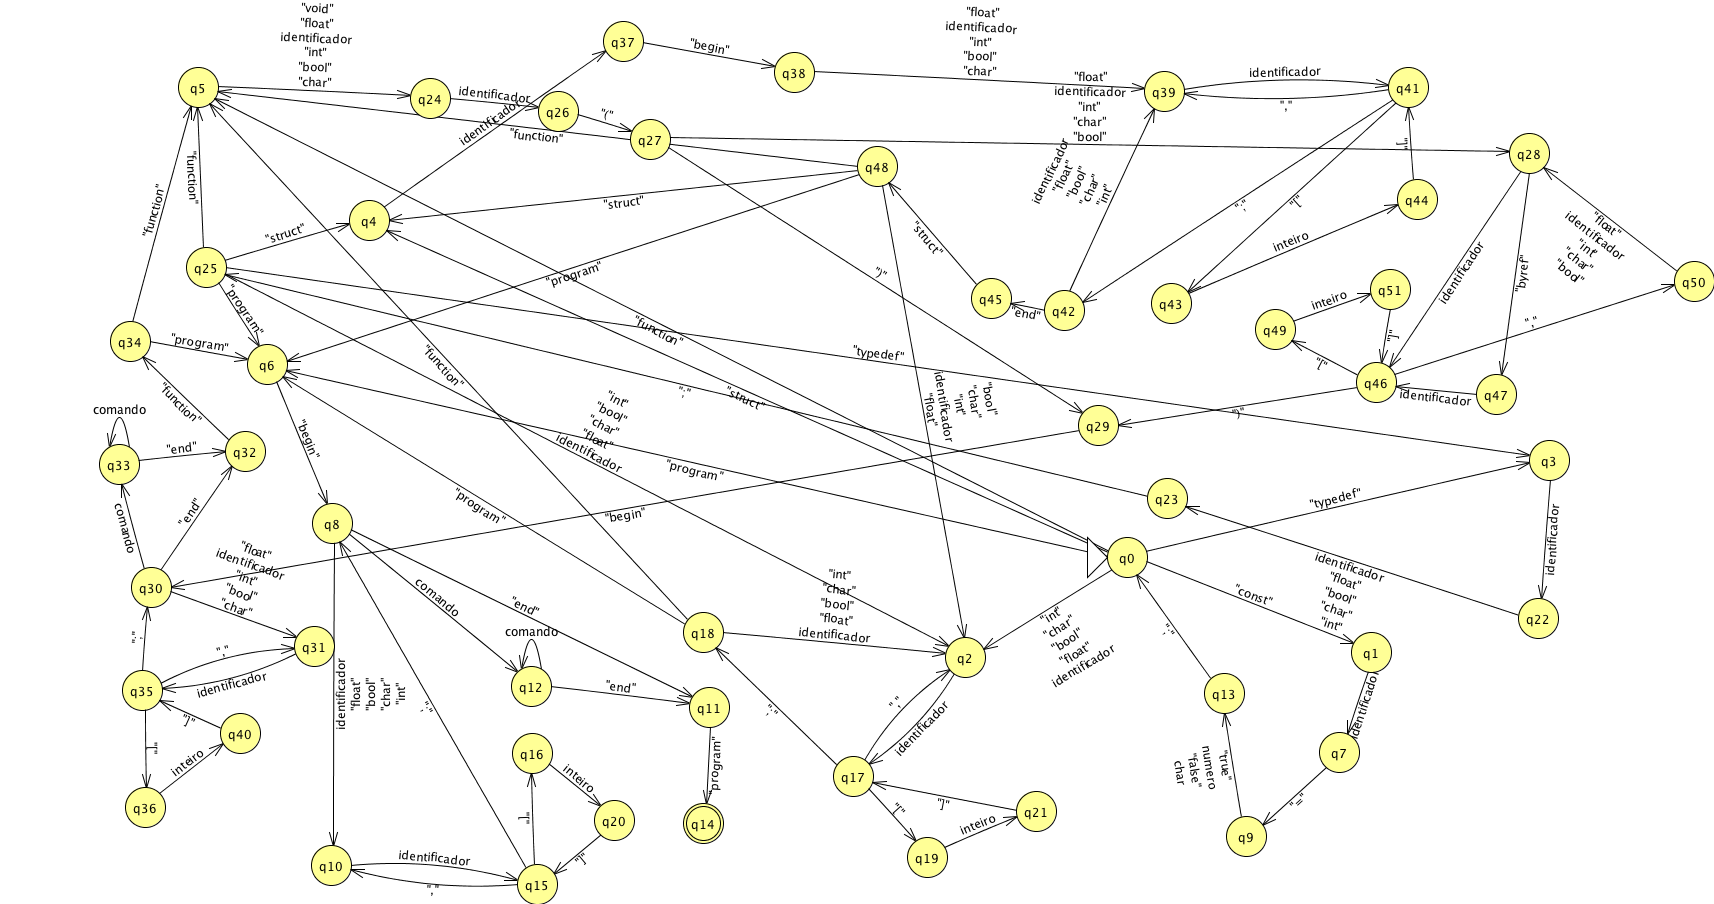
\includegraphics[width=0.7\textwidth]{../1-linguagem/notacoes/JFLAP/programa/programa.png}
      \end{figure}

      \begin{figure}[H]
        \caption{Autômato representando a submáquina comando}
        \centering
          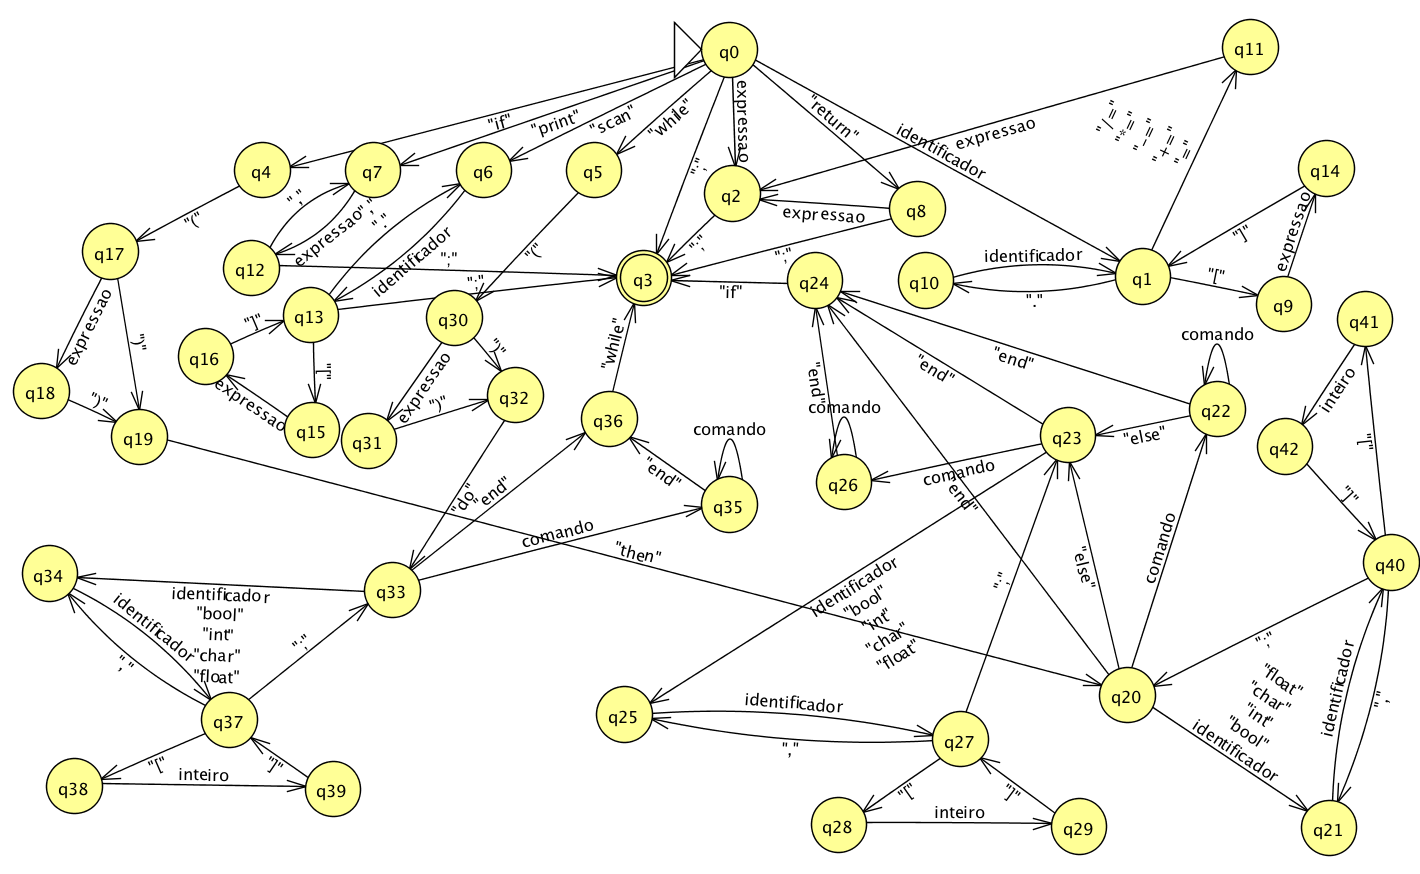
\includegraphics[width=0.7\textwidth]{../1-linguagem/notacoes/JFLAP/comando/comando.png}
      \end{figure}


      \begin{figure}[H]
        \caption{Autômato representando a submáquina expressao}
        \centering
          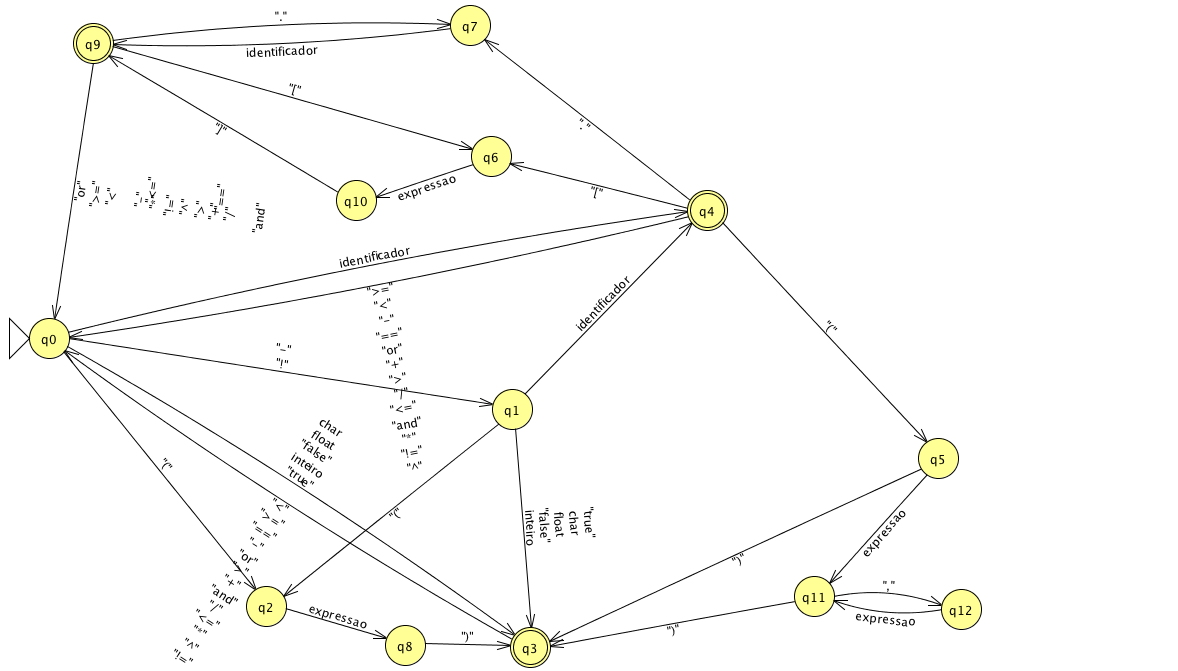
\includegraphics[width=0.7\textwidth]{../1-linguagem/notacoes/JFLAP/expressao/expressao.png}
      \end{figure}

\chapter{Comentários sobre a implementação}

  \section{Desenvolvimento do módulo sintático}

  \section{Integração com o compilador}


\end{document}
